\documentclass{article}
\usepackage{amsmath, amssymb, amsthm, amsfonts}
\usepackage{fullpage}
\usepackage{graphicx}

\newtheorem{theorem}{Theorem}
\newtheorem{lemma}{Lemma}
\newtheorem{corollary}{Corollary}
\newtheorem{definition}{Definition}
\newtheorem{proposition}{Proposition}
\newtheorem{procedure}{Procedure}
\newtheorem{construction}{Construction}
\newtheorem{example}{Example}
\newtheorem{remark}{Remark}
\newtheorem{claim}{Claim}

\newcommand{\Rea}{{\mathbb R}}
\newcommand{\Int}{{\mathbb Z}}
\newcommand{\Rat}{{\mathbb Q}}
\newcommand{\Cmp}{{\mathbb C}}
\newcommand{\Nat}{{\mathbb N}}

\setlength{\oddsidemargin}{.25in}
\setlength{\evensidemargin}{.25in}
\setlength{\textwidth}{6.25in}
\setlength{\topmargin}{-0.0in}
\setlength{\textheight}{8.9in}

\renewenvironment{proof}{\noindent{\bf Proof:} \hspace*{1mm}}{
	\hspace*{\fill} $\Box$ }
\newenvironment{proof_of}[1]{\noindent {\bf Proof of #1:}
	\hspace*{1mm}}{\hspace*{\fill} $\Box$ }
\newenvironment{proof_claim}{\begin{quotation} \noindent}{
	\hspace*{\fill} $\diamond$ \end{quotation}}

\newcommand{\handout}[6]{
   \renewcommand{\thepage}{#1-\arabic{page}}
   \noindent
   \begin{center}
   \framebox{
      \vbox{
    \hbox to 5.78in { {\bf #2} \hfill #3 }
       \vspace{4mm}
       \hbox to 5.78in { {\Large \hfill #4  \hfill} }
       \vspace{2mm}
       \hbox to 5.78in { {\it #5 \hfill #6} }
      }
   }
   \end{center}
   \vspace*{4mm}
   \medskip {\large \noindent {\bf NOTE: } \bf The content of these notes has not been formally reviewed by the lecturer. It is recommended that they are read critically.}
}

\newcommand{\lecture}[3]{\handout{#1}{Ubinet, Distributed Optimization and Games 2016-2017}{#2}{Lecture #1}{Lecturer: Giovanni Neglia}{Scribe: #3}}




\newcommand{\x}{\mathbf{x}}
\newcommand{\y}{\mathbf{y}}
\newcommand{\z}{\mathbf{z}}
\newcommand{\blambda}{\boldsymbol{\lambda}}
\newcommand{\bmu}{\boldsymbol{\nu}}
\usepackage{color}
\usepackage{tikz}
\usepackage{pgfplots}
\usetikzlibrary{positioning}
\usetikzlibrary{arrows}
\usepackage[margin=1in]{geometry}
\usepackage{multirow,booktabs}
\usepackage{dsfont}
\usepackage{subfig}
\usepackage{algorithm}
\usepackage[noend]{algpseudocode}
\graphicspath{ {images/} }


\begin{document}
\lecture{4}{January 11, 2017}{Miguel Romero, Melissa Sanabria}

%Notes
\section{Introduction}
During the previous lecture we studied the dynamics of the bandwidth sharing over a network. For this analysis we took a non-rigorous approach when we assumed that the system must come to a halt (Lec. 3, Sec. 4.2), this reasoning led us to the conclusion that if the system stops it will do it at the optimum, but so far we don't know if the system really stops.

For this reason, in this lesson we will study the convergence of this dynamic system at the limit. In Section 2, we will study the behavior of the rates in some simple network configurations to observe if they eventually converge. We will find that the analysis of the rates in the network is not useful to determine if the system stops. Then, in Section 3, we will evaluate a different function from the system that will help us to determine whether the system stops and if it stops at the optimum.
In Section 4, we will present the simulated annealing process that is a technique that will be utile to find the global optimum of a given function.

\section{Does the system stop?}

In the previous lecture we modeled the ``Bandwith sharing over the Internet'' problem as follows:

\begin{equation}
\begin{aligned}
& \underset{\x , \y }{\text{maximize}}
& &  \sum_{r \in R} U_{r}(x_{r})- \sum_{l \in E} M_{l}(y_{l})\\
& \text{subject to}
& & \ y_l=\sum\limits_{r | l \in r} x_r \\
&      &&  x_{r} \geq 0,\ \forall r \in R\\
\end{aligned}
\label{eq1}
\end{equation}

If we solve this problem by the Lagrange multipliers method, the optimal solution is:

\begin{equation}
\ U'_{\bar r}(x^*_{\bar r})
\begin{cases}
= \sum_{l \in {\bar r}} M'_l(y^*_{l})  & \mbox{if } x^*_{\bar r} > 0,\\ 
\leq \sum_{l \in {\bar r}} M'_l(y^*_{l}) & \mbox{if }x^*_{\bar r} = 0.
\end{cases}
\label{eq2}
\end{equation}

This problem can be also solved using a distributed approach, where each network component has a role:
\begin{itemize}
\item The links measure congestion and transmit to the sources all the flow passing by them.
\item The sources should adapt their rate over time according to the following equation:
\begin{equation}
\frac{dx_r}{ dt}=k_r(U'_r(x_r(t)) - \sum_{l \in {r}} M'_l(y_l(t) )   )
\label{eq3}
\end{equation}
\end{itemize}

We have concluded that if the elements of the network follow this dynamic and the system stops (the sources eventually stop changing their rate), then they stop at a point where the derivative (equation \eqref{eq3}) is equal to zero. Because otherwise, if the derivative is not zero, means that the system keeps changing.

If this derivative is equal to zero, then, from equation \eqref{eq3}, we get:

\begin{equation}
U'_r(x_r(t)) = \sum_{l \in {r}} M'_l(y_l(t))
\label{eq4}
\end{equation}

We recognize, this is the same equation as the (strictly positive) optimal solution obtained by the lagrange multipliers method (equation \eqref{eq2}); but so far we have assumed that the system stops, let's observe with a few examples if the system actually stops.

\subsection{First example: A single link with only one route}

Let's first see the case of a single link with a single route, illustrated in Figure~\ref{figur1}.

\begin{figure}[h!]
\centering
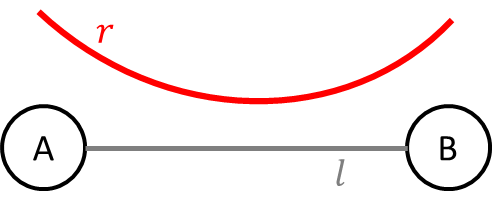
\includegraphics[scale=.7]{1Link1Route}
\caption{A single link with one route.}
\label{figur1}
\end{figure}

Assume that the equation of this network leads to the following:

\begin{equation}
\frac{dx_r}{dt}=k_r(1 - y_{l})
\label{eq5}
\end{equation}

But, as there is only one route, we have $y_{l}=\sum\limits_{r | l \in r} x_r=x_{r}$, then:

\begin{equation}
\frac{dx_r}{dt}=k_r(1 - x_{r})
\label{eq6}
\end{equation}

The general solution of this differential equation is:

\begin{equation}
x_{r}(t)= 1 + a e^{-k_{r} t}
\label{eq7}
\end{equation}

Imposing the initial condition $x_{r}(0)=0$, we get that $a=-1$ and then we arrive to the solution:

\begin{equation}
x_{r}(t)= 1 - e^{-k_{r} t}
\label{eq8}
\end{equation}

We observe in Figure~\ref{figur2} that this solution approaches to $1$ exponentially fast, and in particular, it happens that the value of $k_r$ is the slope of the curve, it means that if $k_r$ is big, it grows fast.

\begin{figure}[h!]
\centering
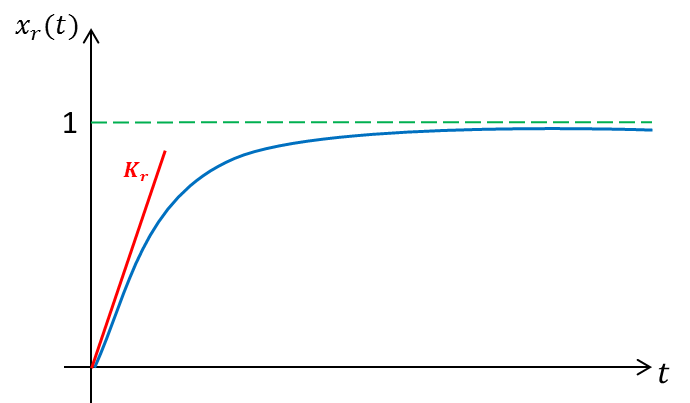
\includegraphics[scale=.7]{rIn1Route}
\caption{Dynamics of rate in route $r$.}
\label{figur2}
\end{figure}

Now, if we would like to solve our original maximization problem (equation \eqref{eq1}), we need the values of $U_{r}(x_{r})$ and $M_{l}(y_{l})$.
From equation \eqref{eq3} and equation \eqref{eq5} we can deduce that:

\begin{equation}
U_{r}'(x_r) = 1 \implies U_{r}(x_r)=x_r
\label{eq9}
\end{equation}

\begin{equation}
M_l'(y_l) = y_l \implies M_{l}(y_l)=\frac{{y_l}^2}{2}
\label{eq10}
\end{equation}

Then, the maximization problem is:

\begin{equation}
\begin{aligned}
& \underset{\x, \y}{\text{maximize}}
& &  x_{r} - \frac{{y_l}^2}{2}\\
& \text{subject to}
& & \ y_l=x_r \\
&      &&  x_{r} \geq 0,\ \forall r \in R\\
\end{aligned}
\label{eq11}
\end{equation}

Using the first constraint we can directly replace the value of $y_l$ by $x_r$.

\begin{equation}
\begin{aligned}
& \underset{\x, \y}{\text{maximize}}
& &  x_r - \frac{{x_r}^2}{2}\\
& \text{subject to} & & \ x_{r} \geq 0,\ \forall r \in R\\
\end{aligned}
\label{eq12}
\end{equation}

Using equation \eqref{eq9} and \eqref{eq10}, in the solution of the optimization problem (equation \eqref{eq2}), we get:

\begin{equation}
\ 1
\begin{cases}
= x^*_r  & \mbox{if } x^*_{r} > 0,\\ 
\leq x^*_r & \mbox{if } x^*_{r} = 0.
\end{cases}
\label{eq13}
\end{equation}

This equations tell us that either 
$$\begin{cases}
x^*_r = 1 \land x^*_r > 0  \implies x^*_r = 1\\
x^*_r \geq 1 \land x^*_r = 0 \implies \textbf{contradiction}
\end{cases}$$

Then, the optimal rate for this problem is $x^*_r = 1$.
So, in this original problem, the source should transmit at rate 1.

We can observe, going back to the solution of the differential equation (equation \eqref{eq8}), that you go to this optimum $x^*_r = 1$, but the more you approach it the less is the speed at which you go there, then the convergence is asymptotic, you are decreasing your speed, but you are never stopping at the optimum.

\subsection{Second example: Two routes sharing a link}

We have seen until now that we converge to the optimum asymptotically, but although we are not stopping at the optimum, we are approaching it continuously, now we would like to see if this is always the case. Let's analyze a second example (illustrated in Figure~\ref{figur3}), in which we observe the behavior of the rates in two routes using the same link.

\begin{figure}[h!]
\centering
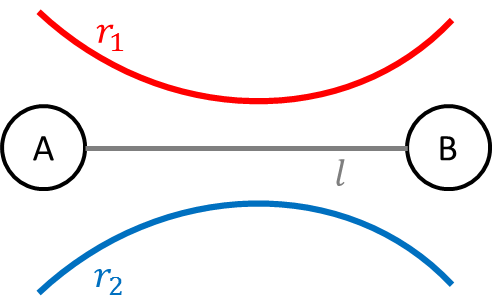
\includegraphics[scale=.7]{1Link2Routes}
\caption{Two routes sharing a link.}
\label{figur3}
\end{figure}

Assume that these are the equations of the flows:

\begin{equation}
\frac{dx_{r_1}}{dt}=k_{r_1}(\frac{1}{x_{r_1}} - y_{l})
\label{eq14}
\end{equation}
\begin{equation}
\frac{dx_{r_2}}{dt}=k_{r_2}(\frac{2}{x_{r_2}} - y_{l})
\label{eq15}
\end{equation}

We can deduce the Utility functions of these flows as we have done for the previous example:

\begin{equation}
U_{r_1}'(x_{r_1}) = \frac{1}{x_{r_1}} \implies U_{r_1}(x_{r_1})=\ln{x_{r_1}}
\label{eq16}
\end{equation}
\begin{equation}
U_{r_2}'(x_{r_2}) = \frac{2}{x_{r_2}} \implies U_{r_2}(x_{r_2})=2\ln{x_{r_2}}
\label{eq17}
\end{equation}

We can also deduce the Cost function of the link:

\begin{equation}
M_l'(y_l) = y \implies M_l(y_l) = \frac{y^2}{2}
\label{eq18}
\end{equation}

\subsubsection{$r_1$ alone}
First, let's assume that at the beginning ${r_1}$ is alone, then developing a similar procedure as for the previous example, the condition would be:

\begin{equation}
\ \frac{1}{x^*_{r_1}}
\begin{cases}
= x^*_{r_1}  & \mbox{if } x^*_{r_1} > 0,\\ 
\leq x^*_{r_1} & \mbox{if } x^*_{r_1} = 0.
\end{cases}
\label{eq19}
\end{equation}

This equations tells us that either 
$\begin{cases}
{x^*_{r_1}}^2 = 1 \land x^*_{r_1} > 0 \implies x^*_{r_1} = 1\\
{x^*_{r_1}}^2 \geq 1 \land x^*_{r_1} = 0 \implies \textbf{contradiction}
\end{cases}$

Then, the optimal value is $x^*_{r_1} = 1$.

\subsubsection{$r_1$ and $r_2$ together}
Now, let's look at the case where ${r_1}$ and ${r_2}$ are together. We can deduce the Utility function of these flows as follows, for ${r_1}$:

\begin{equation}
\ U'_{r_1}(x^*_{r_1})
\begin{cases}
= M'_l(y^*_{l})  & \mbox{if } x^*_{r_1} > 0,\\ 
\leq M'_l(y^*_{l}) & \mbox{if } x^*_{r_1} = 0.
\end{cases}
\label{eq20}
\end{equation}

As we know that $U_{r_1}'(x_{r_1}) = \frac{1}{x_{r_1}}$ and $M_l'(y_l) = y_{l}=\sum\limits_{r | l \in r} x_r=x_{r_1}+x_{r_2}$, then, replacing:

\begin{equation}
\ \frac{1}{x_{r_1}}
\begin{cases}
= x^*_{r_1}+x^*_{r_2}  & \mbox{if } x^*_{r_1} > 0,\\ 
\leq x^*_{r_1}+x^*_{r_2} & \mbox{if } x^*_{r_1} = 0.
\end{cases}
\label{eq21}
\end{equation}

Similarly for ${r_2}$:

\begin{equation}
\ \frac{2}{x_{r_2}}
\begin{cases}
= x^*_{r_1}+x^*_{r_2}  & \mbox{if } x^*_{r_2} > 0,\\ 
\leq x^*_{r_1}+x^*_{r_2} & \mbox{if } x^*_{r_2} = 0.
\end{cases}
\label{eq22}
\end{equation}

Let's suppose that $x^*_{r_1} > 0$ and $x^*_{r_2} > 0$, then we have a system of two equations:

\begin{equation}
\frac{1}{x^*_{r_1}} = x^*_{r_1}+x^*_{r_2}
\label{eq23}
\end{equation}

\begin{equation}
\frac{2}{x^*_{r_2}} = x^*_{r_1}+x^*_{r_2}
\label{eq24}
\end{equation}

Subtracting equations \eqref{eq23} and \eqref{eq24}:

\begin{equation}
\frac{1}{x^*_{r_1}} - \frac{2}{x^*_{r_2}} = 0 \implies x^*_{r_2}=2x^*_{r_1}
\label{eq25}
\end{equation}

Using equation \eqref{eq25} in equation \eqref{eq23}, we get:
\begin{equation}
{3x^*_{r_1}}^2=1 \implies x^*_{r_1}=\frac{1}{\sqrt{3}}
\label{eq26}
\end{equation}

Replacing equation \eqref{eq26} in equation \eqref{eq25}:
\begin{equation}
x^*_{r_2}=\frac{2}{\sqrt{3}}
\label{eq27}
\end{equation}

This result is coherent, because as they are sharing the same link and the utility of $r_2$ is higher than the utility of $r_1$, is reasonable that at the end (in the optimal case) the rate of $r_2$ is higher than the rate of $r_1$.

Now with this information, we can try to see what can be the dynamics of the rates.

\subsubsection{Dynamics $r_1$ alone}
Let's start trying to deduce the dynamics of $x_{r_1}$ for the first case. When $r_1$ is alone, it will converge to 1, we don't know the exact shape, but it can be similar to the one presented in Figure~\ref{figur4}.

\begin{figure}[h!]
\centering
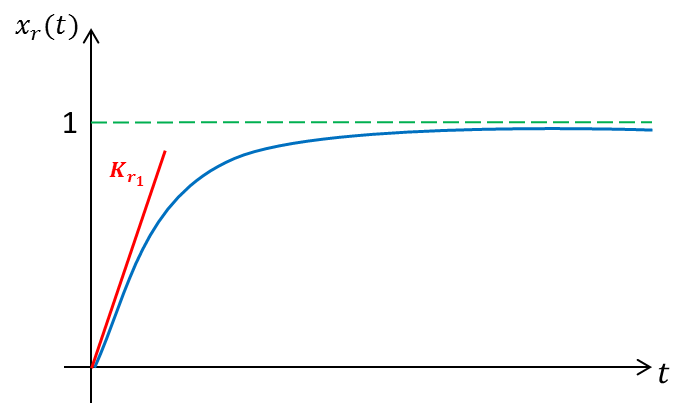
\includegraphics[scale=.6]{r1Alone}
\caption{Behavior of $r_1$ alone.}
\label{figur4}
\end{figure}

In particular, the speed at which it approaches 1 will be related to $k_{r_1}$.

\subsubsection{Dynamics $r_1$ and $r_2$ together}
Now, let's take a look to the behavior of $x_{r_1}$ and $x_{r_2}$ when $r_1$ and $r_2$ are sharing the link. In this case, it is more complex to know what will happen, because $x_{r_1}$ has its target in $\frac{1}{\sqrt{3}}$ and the target of $x_{r_2}$ is $\frac{2}{\sqrt{3}}$. Again, the speed at which they approach to their targeted value will depend on the parameter $k_{r_1}$ and $k_{r_2}$.

Let's assume that $k_{r_2}$ is much smaller than $k_{r_1}$:

\centerline{$k_{r_2} << k_{r_1}$}

so that $x_{r_2}$ changes but very slowly.

\begin{figure}[h!]
\centering
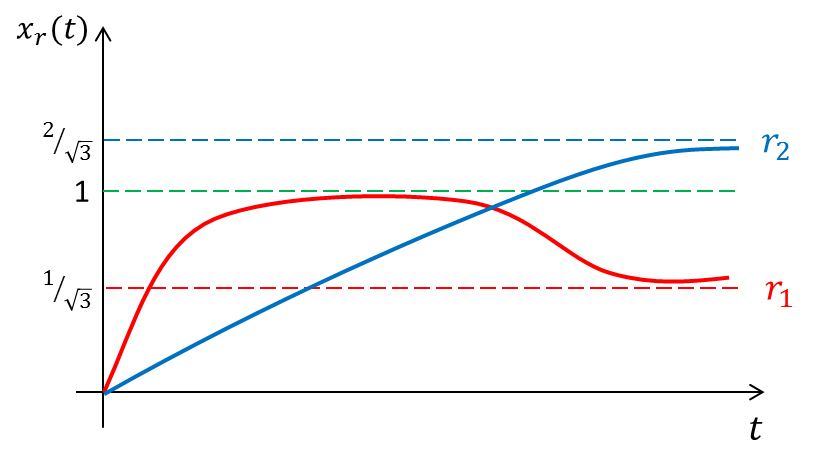
\includegraphics[scale=.6]{r1Andr2Together}
\caption{Behavior of $r_1$ and $r_1$ together.}
\label{figur5}
\end{figure}

So, as illustrated in Figure~\ref{figur5}, at the beginning the influence of $r_2$ will be so low that $r_1$ will not notice it, and then $r_1$ will start to increase its rate, $x_{r_1}$ will tend to go to 1, as if it were alone in the link.

Meanwhile $r_2$ will be increasing its rate slowly. At one point $x_{r_2}$ will start becoming significant, and the more $x_{r_2}$ grows, the more $x_{r_1}$ will start perceiving the congestion, until $x_{r_1}$ has to come back to its final (optimal) condition.

We can see that actually, even if there are only two flows sharing the link, it is possible that at the beginning one of them overshoots its target to perhaps come back later, and these dynamics could be even more complex as we will see with the following examples.

\subsection{Third example: More complex networks}

We have seen that for a simple network with only one link and two routes sharing the link, the equations and the behavior of the flows start to be complex, now, let's take a look to the configuration shown in Figure~\ref{figur6}, where $r_1$ and $r_2$ are competing for link $l_2$, and $r_2$ and $r_3$ are competing for link $l_3$.

\begin{figure}[h!]
\centering
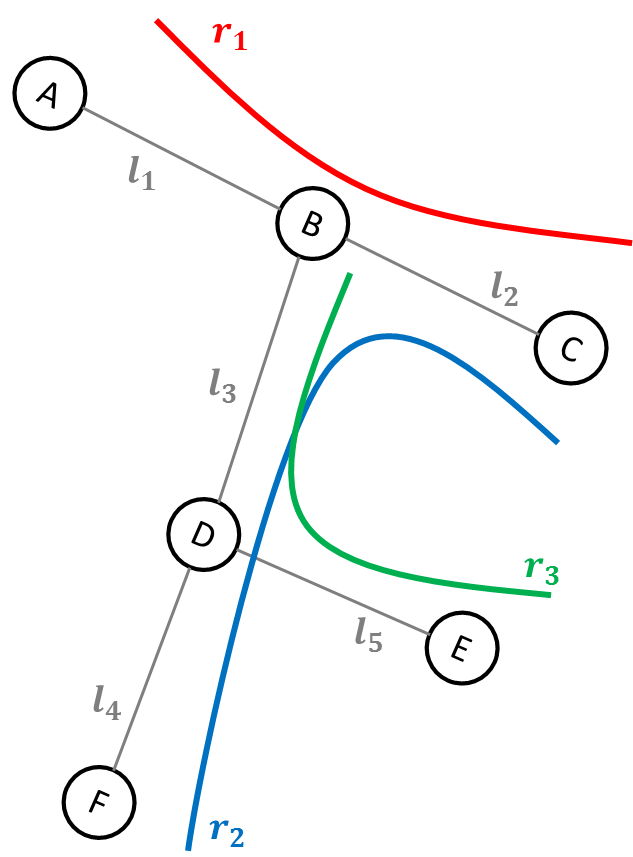
\includegraphics[scale=.7]{NLink3Routes}
\caption{Example of a network configuration with 3 routes over 5 links.}
\label{figur6}
\end{figure}

Let's say that the utilities of the sources $r_1$, $r_2$, and $r_3$ are the following:
\begin{equation}
\begin{aligned}
&U_{r_1}(x_{r_1})=\ln{x_{r_1}} \\
&U_{r_2}(x_{r_2})=2\ln{x_{r_2}} \\
&U_{r_3}(x_{r_3})=10\ln{x_{r_3}}
\end{aligned}
\label{eq28}
\end{equation}

Now, assume that $k_{r_1} >> k_{r_2} >> k_{r_3}$. In Figure~\ref{figur7} we observe the possible behavior of flow $x_{r_1}$: At the beginning $x_{r_1}$ will grow pointing to 1, when $x_{r_2}$ starts to be significant, $x_{r_1}$ will start to decrease towards $\frac{1}{\sqrt{3}}$, but then after some time, $x_{r_3}$ will be high enough to compete with $x_{r_2}$ on link $l_3$, and because it has larger utility, it will probably reduce the rate of $r_2$. Then $r_1$ will have more space on link $l_2$, and will increase its rate again approaching to 1, and the dynamics continue.

\begin{figure}[h!]
\centering
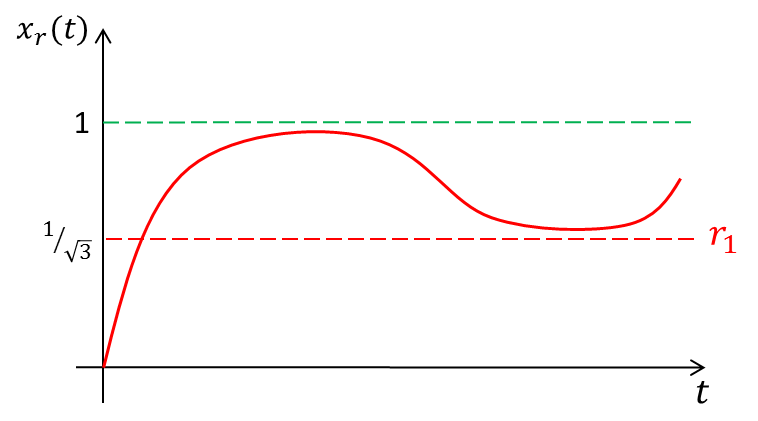
\includegraphics[scale=.7]{r1In3Routes}
\caption{Flow $x_{r_1}$ over time.}
\label{figur7}
\end{figure}

Then we can build a more complex network configuration like the one proposed in Figure~\ref{figur8}, where it is possible that a behavior like the following occurs: 
First $x_{r_1}$ will grow towards 1, then $x_{r_2}$ starts to be significant, and $x_{r_1}$ decrease approaching its goal value. After some time, $x_{r_3}$ will be noticed by $x_{r_2}$ which will reduce its own rate, causing that $x_{r_1}$ increases again. At some point, $x_{r_4}$ will be perceived by $x_{r_3}$ which will reduce its own rate, this will yield the increasing of $x_{r_2}$ and consequently the reduction of $x_{r_1}$. In general, the dynamics will continue running and the rates can oscillate going up and down, now it's not clear anymore even if they asymptotically converge to an equilibrium point.

\begin{figure}[h!]
\centering
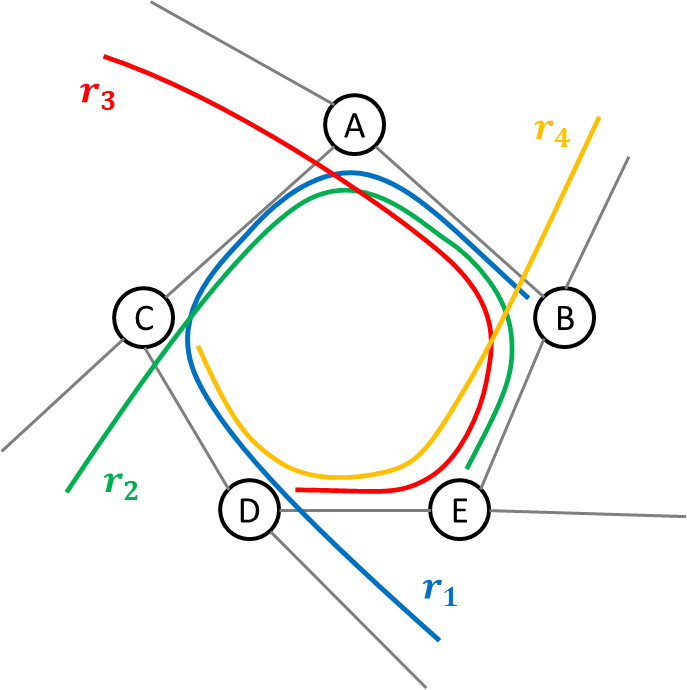
\includegraphics[scale=.7]{complexNetwork}
\caption{Network configuration with 10 links and 4 flows.}
\label{figur8}
\end{figure}

\section{Does the system converge?}
We wanted to find something like the following:
$$\lim_{t\to\infty} x_r(t) = x^*_r$$

In general: given a system of equations:
$$\dot{x}_{r_1}(t) = f_1(x_{r_1}, x_{r_2})$$
$$\dot{x}_{r_2}(t) = f_2(x_{r_1}, x_{r_2})$$

We would like to prove that:
$$\dot{x}_{r_1}(t) \xrightarrow[t\to\infty]{} x^*_{r_1}$$
$$\dot{x}_{r_2}(t) \xrightarrow[t\to\infty]{} x^*_{r_2}$$

One possibility to prove this is to observe the variable $x_{r_1}$ over time, and show that it is each time closer to $x^*_{r_1}$, then do the same for $x^*_{r_2}$. Once you have proven that each of the variables $x_{r}$ in the system converge to $x^*_{r}$ over time, the prove is finished.

What we have seen is that it is not possible to use this proof method, because from the study of the flows in the previous section we have observed the following:
\begin{itemize}
\item Probably the system will not converge in finite time.
\item It is possible that we are in a chaotic system. We are not sure if the system will eventually converge.
\end{itemize}

Instead of analysing the rates, because as we have seen in the previous section they can oscilate, and it is not clear how this can lead us to some convergence, we want to use another function that helps us.

We can think here on the function we used in the maximization problem:

\begin{equation}
\begin{aligned}
V(t) = \sum_{r \in R} U_{r}(x_{r}(t))- \sum_{l \in E} M_{l}(y_{l})\\
\end{aligned}
\label{eq29}
\end{equation}

We can wonder, is it possible that although each individual rate does not go closer and closer over time to the optimal solution, this global function (equation \eqref{eq29}) keeps going closer and closer to the optimal solution? 

To answer this, we have to solve two questions:
\begin{enumerate}
\item Does $V(t)$ always increase unless it reaches the optimum?
$$\frac{dV(t)}{dt} > 0,\ \forall t \ \ unless \  V(t) = \max V(x_r) \ ?$$
\item Does this function achieve the point of maximum?
$$\lim_{t\to\infty} V(t) = \max V(x_r) \ ?$$
\end{enumerate}

If the answers to this two questions are Yes, imply that:

$$\lim_{t\to\infty} x_r(t) = x_r^*$$

Because $x_r^*$ is the only point where the function $V(t)$ is maximum, and if $V(t)$ is always increasing, then once it reaches the maximum, it cannot continue changing/increasing more over time.

We will use the following additional hypothesis:

$$U'_r(0) = +\infty,\ \forall r \in R$$

If this is true, then we know that $x_r^* > 0$, and it means that we can only consider the simplest equations (equality equations) in the condition of equation \eqref{eq2}.

\subsection{Is $V(t)$ always increasing?}
To know if the function $V(t)$ is increasing with time, we compute the derivative (using the chain rule):

\begin{equation}
\begin{aligned}
\frac{dV(t)}{dt} = \frac{dV(x_{r_1}(t), x_{r_2}(t), ... , x_{r_R}(t))}{dt}= \sum_{r \in R} \frac{\partial V}{\partial x_r} \cdot \frac{dx_r}{dt}
\end{aligned}
\label{eq30}
\end{equation}

Computing the partial derivative $\partial V/\partial x_r$:

\begin{equation}
\begin{aligned}
\frac{\partial V}{\partial x_r} = (U'_r(x_r(t)) - \sum_{l \in {r}} M'_l(y_l(t)))
\end{aligned}
\label{eq31}
\end{equation}

And we already had the result of $dx_r/dt$ in equation \eqref{eq3}. Then replacing \eqref{eq3} and \eqref{eq31} in \eqref{eq30}:

\begin{equation}
\begin{aligned}
\frac{dV(t)}{dt} = \sum_{r \in R} (U'_r(x_r(t)) - \sum_{l \in {r}} M'_l(y_l(t)))^2 \cdot (k_r)
\end{aligned}
\label{eq32}
\end{equation}

We have the squared term of ($U'_r(x_r(t)) - \sum_{l \in {r}} M'_l(y_l(t))$), multiplied by a positive term ($k_r$), and then we have the sum over these positive terms, then we can conclude that the value of $dV(t)/dt$ is always positive. 

\begin{equation}
\begin{aligned}
\frac{dV(t)}{dt} \geq 0,\ \forall t
\end{aligned}
\label{eq33}
\end{equation}

If we check the point where the derivative is equal to zero:

\begin{equation}
\begin{aligned}
\frac{dV(t)}{dt} = 0 \implies U'_r(x_r(t)) = \sum_{l \in {r}} M'_l(y_l(t))
\end{aligned}
\label{eq34}
\end{equation}

We can remember from equation \eqref{eq2} that this is the same optimal solution obtained by the method of lagrange multipliers. It implies a much stronger condition, this function is always increasing unless we arrive to the optimum:

\begin{equation}
\begin{aligned}
\frac{dV(t)}{dt} > 0,\ \forall t \ \ unless \  x_r(t) = x_r^*(t)
\end{aligned}
\label{eq35}
\end{equation}

\subsection{Does $V(t)$ go towards $V(x^*)$?}
Now the question that arises is, does $V(t)$ go towards $V(x^*)$?

Because it could be that the function is increasing but each time slower that it approaches assymptotically to the optimum, and never reaches it.

So, what does it mean that the function $V(t)$ never reaches the maximum?
Let's try to illustrate the space of $x_r$ in Figure~\ref{figur9}.

\begin{figure}[h!]
\centering
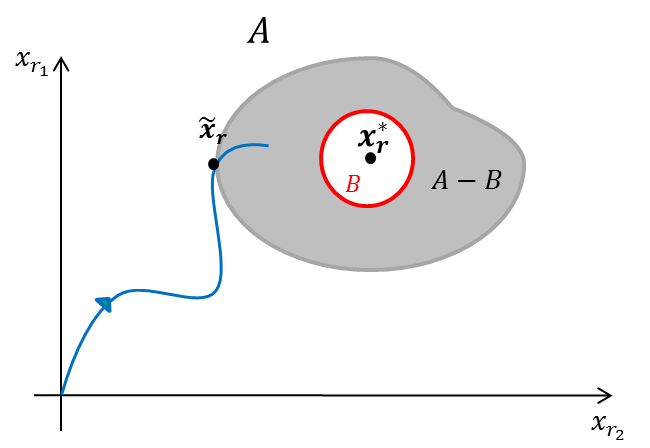
\includegraphics[scale=.7]{ball}
\caption{Evolution (over time) of $x_r$ in the space, plot for two routes, $R = {r_1,r_2}$.}
\label{figur9}
\end{figure}

This Figure plots the evolution over time of the values of $x_r$, then we start from $x_r = 0$, and we target to the optimum (it can be targeted in a strange way as shown in the figure), this is the curve over time, and let's suppose it approaches assymptotically to $x_r^*$.

At one instant we will be at point $\widetilde{x}_r$, now let's define the set $A$ to be:

\begin{equation}
\begin{aligned}
A = \{{x}_r\ \mid\ V({x}_r) \geq V(\widetilde{x}_r) \}
\end{aligned}
\label{eq36}
\end{equation}

The set $A$ will include $\widetilde{x}_r$ and $x^*_r$ (the optimum), as shown in Figure~\ref{figur6}. This set is compact (closed and bounded).

Let's assume now that we are approaching $x^*_r$ asymptotically, this means that we will never reach it, and then there will exist a ball $B$ around $x^*_r$ such that ${x}_r(t)$ will never be there at any time.

\begin{equation}
\begin{aligned}
\mbox{If } {x}_r(t) \not\to x^*_r \implies \exists \ B\ \mid\ {x}_r(t) \not\in B\ \forall t
\end{aligned}
\label{eq37}
\end{equation}

Now, if we look at the set $A-B$, we find that in this set, $dV/dt$ is strictly positive, because we already found that this derivative is always positive, except in $x^*_r$ and this point does not belong to the set $A-B$.

$$\frac{dV}{dt} > 0\ \mbox{  over } A-B$$

Then, the function $dV/dt$ happens to be continuous, and we have seen that set $A$ is a compact set. 
\begin{claim}
A continuous function over a compact set implies that the function has a maximum and a minimum on the set.
\end{claim} 
This is telling us that $V(t)$ moves inside $A-B$ with a strictly positive speed ($a$).

$$\frac{dV}{dt} \ \mbox{is continuous over a compact set}\ \implies\ \exists \min \frac{dV}{dt} = a > 0$$

This implies that $V(t)$ cannot stay forever out of set $B$. In other words, it cannot be that $V(t)$ is always increasing but it never goes inside set $B$. Then we arrived to a contradiction, because we supposed that $V(t)$ could have stayed always inside the set A-B and we found that it does not happen.

Our proof is finished. Then we can conclude that:
\begin{remark}
We started from an optimization problem, and we have shown that the dynamics we have defined converge to the optimum.
\end{remark}
\begin{remark}
From another point of view, if you don't have the optimization problem, but you have the dynamics of the system, and you wonder if they converge or not. We can prove it by defining a real function that always increases. This function is usually called "potential function" or "Lyapunov function".
\end{remark}


\section{Simulated Annealing | GIBBS Sampling}

Annealing is a heat process whereby a metal is heated to a specific temperature and then allowed to cool down slowly. This softens the metal which means it can be cut and shaped more easily.

The idea of this procedure is to heat the metal in order to cause the oscillation of the atoms which will potentially break the disordered pieces of the metal. The temperature is slowly reduced to make the atoms move until they reach some ordered state, which is the minimum energy configuration.  

If this configuration has the minimum energy configuration, the question is why the metal by itself does not go directly to this configuration? 

It happens because the metal presents an analog situation to the one shown in Figure~\ref{figur10}. This figure represents a system with different states, which can be all the different positions of the atoms in the metal. Let's assume that there is a ball that arrives to this curve in a point (state), and you know there is another state in the system that has less energy, but in order to reach that point, the ball need to pass first through a space where the energy is higher.

\begin{figure}[h!]
\centering
\subfloat[Original State of the system.]{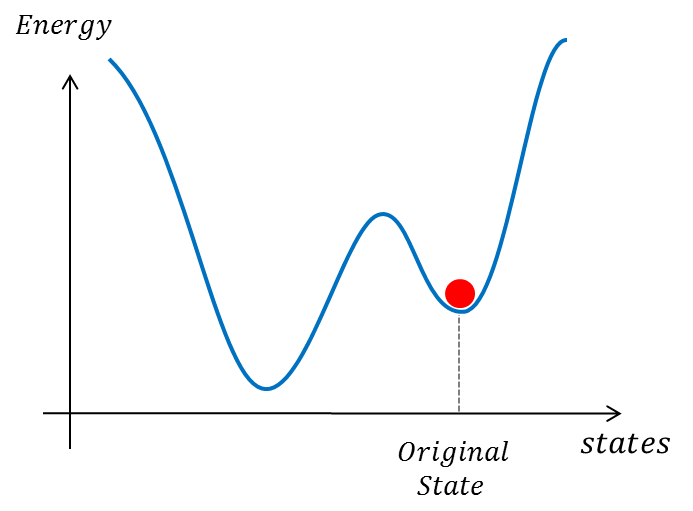
\includegraphics[scale=.5]{originalState}}
\subfloat[Trajectory of the ball from the initial state after aplying some
kinetic force until it arrives to the final state.]{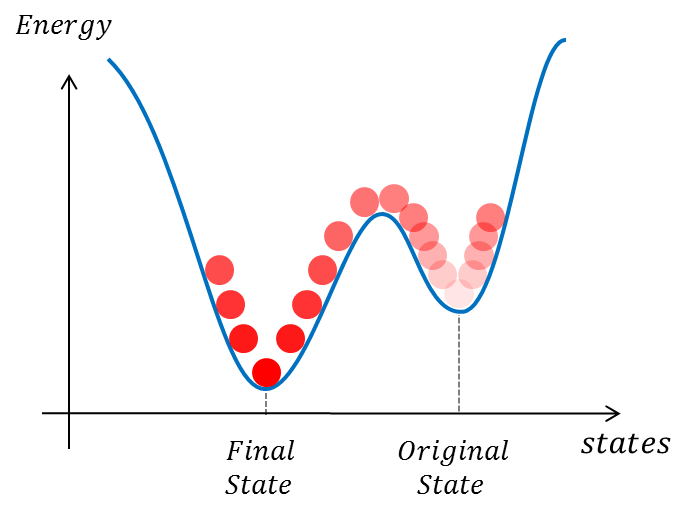
\includegraphics[scale=.5]{trajectory}}
\caption{Energy of the system for the different states.}
\label{figur10}
\end{figure}

If you can increase the kinetic energy of the ball, at one point, the ball will be able to pass by the configuration of higher energy, and then will reach the minimum energy configuration; meanwhile you can reduce gradually the energy until the ball is again motionless, but now in the global minima.

Now, we can formalize the definition of the problem. Let's assume we have a set of states $S$, and a number $N$ of agents. Each agent $i$ has some internal variable $a_i \in  A_i$ where $A_i$ is a finite set. We also define the state as $S(a_1, a_2, ... , a_N)$. Then, if you have a finite number of agents ($N$), and they have a finite number of possibilities ($\mid A_i \mid$), the space is finite (and not continuous as the problems seen in the previous sections).

Let's see an example. Suppose that action $a_i \in \{0,1\}$, and the state of the system is characterized by Equation \ref{eq38} which describe how many nodes have done a particular choice, then a possible plot of this example is presented in Figure~\ref{figur11}.

\begin{equation}
\begin{aligned}
S(a_1, a_2, ... , a_N)=\sum_{i = 1}^{N} \mathds{1}(a_i = 1)
\end{aligned}
\label{eq38}
\end{equation}

\begin{figure}[h!]
\centering
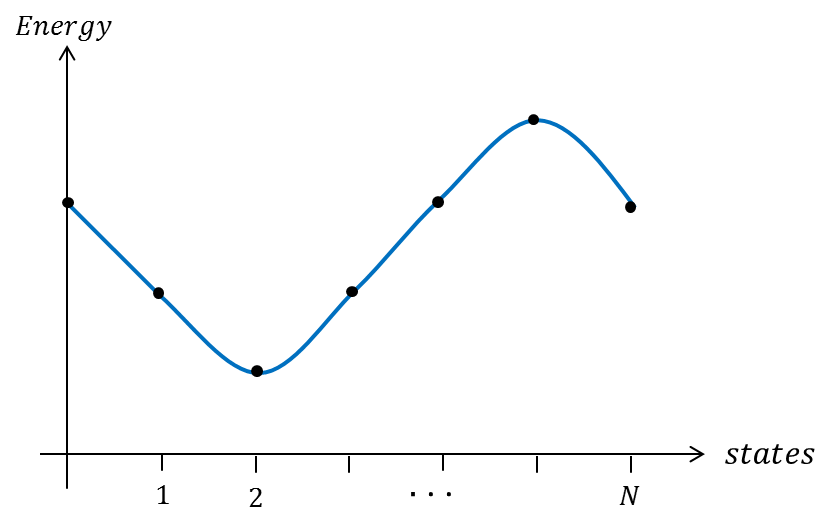
\includegraphics[scale=.5]{statesVsEnergy}
\caption{State of the system.}
\label{figur11}
\end{figure}

To solve this simple example, we want to minimize the energy $\xi$ that is a function of state $S$ (Equation \ref{eq39}), the goal is to find the state for which the energy is minimal.

\begin{equation}
\begin{aligned}
& \underset{\{a_{i}\}}{\text{minimize}}
& &  \xi(S(a_1,...,a_N))\\
\end{aligned}
\label{eq39}
\end{equation}

There are some strong differences with the problems we solved before. Now, the solution space is finite and we do not rely on assumptions about the shape of the function (concave, convex, increasing, etc).

\subsection{Neighborhood Relation}

One way to solve the problem described before is to have a neighborhood relation, meaning that from one state you can consider some other state. This relation is shown in Figure~\ref{figur12} where we can move from state $S_i$ to state $S_j$, but cannot move directly from state $S_i$ to state $S_k$. 

\begin{figure}[h!]
\centering
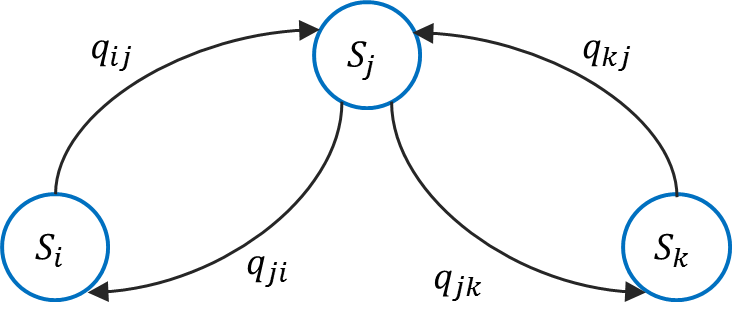
\includegraphics[scale=.5]{neighborhoodRelation}
\caption{Representation of Neighborhood relation.}
\label{figur12}
\end{figure}

First, let's describe some definitions.
\begin{itemize}
\item $q_{ij}$ is the probability of state $S_i$ to consider state $S_j$
\item $\xi(S_j) = \xi_j$ is the energy of state $S_j$
\item $\alpha_{ij}$ is the probability to move from state $S_i$ to state $S_j$ given that you have considered state $S_j$
\end{itemize}

\subsection{Modelling the problem as a Markov Chain}

Now, let's define some rules: 
\begin{enumerate}
\item At every step you can consider one of your neighbors with probability $q_{ij}$.\\
\indent We will assume that $q_{ij} = q_{ji}$.
\item Once you decide to look into node $j$, you can compare its energy with your energy according to Equation \ref{eq40}, where we can observe that if the difference is small, the probability to move to state $S_j$ is high.
\end{enumerate}

\begin{equation}
\ \alpha_{ij} = 
\begin{cases}
1  & \mbox{if } \xi_{j} \leq \xi_{i},\\ 
e^{-\frac{\xi_{j}-\xi_{i}}{T}} & \mbox{if }\xi_{j} > \xi_{i}.
\end{cases}
\label{eq40}
\end{equation}

From (\ref{eq40}) we can observe that if the energy of state $S_j$ is smaller than the energy in the current state, I will always move there. On the other hand, if the energy of state $S_j$ is greater than my current energy, I will move depending on the difference of the energies. If the difference is small, then I would go there with a high probability but if the difference is very large, it will be very unlikely that I move to state $S_j$.

After all this, we have found a Markov chain (Figure~\ref{figur13}), where the probability to go from $S_i$ to $S_j$ is $q_{ij}\cdot \alpha_{ij}$.

\begin{figure}[h!]
\centering
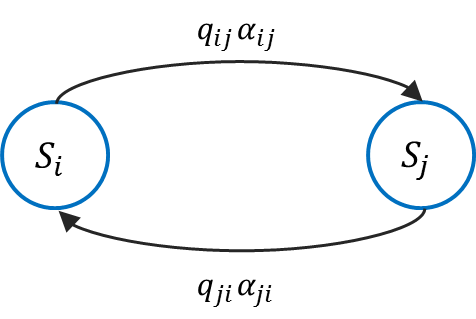
\includegraphics[scale=.5]{markovChain}
\caption{Markov chain.}
\label{figur13}
\end{figure}

If this Markov Chain is reversible, we know that it will converge to the stationary distribution described in (\ref{eq41}), meaning that if we let this markov chain run during a long time, we know that with some probability $\pi_i$ it will be at state $S_i$, if we assume the Markov Chain is reversible, then this probability is:

\begin{equation}
\begin{aligned}
\pi_i = \frac{e^{-{\frac{\xi_i}{T}}}}{\sum_j e^{-\frac{\xi_j}{T}}}
\end{aligned}
\label{eq41}
\end{equation}

To check if (\ref{eq41}) is really the stationary distribution of our problem, we have to proof the reversibility property of this Markov Chain. It means that if we take any two neighbors $S_i$ and $S_j$ the rate at which I go from $S_i$ to $S_j$, ($\pi_i \cdot q_{ij} \cdot \alpha_{ij}$), and the rate at which I go from $S_j$ to $S_i$, ($\pi_j \cdot q_{ji} \cdot \alpha_{ji}$), should be equal:

\begin{equation}
\begin{aligned}
\pi_i \cdot q_{ij} \cdot \alpha_{ij} = \pi_j \cdot q_{ji} \cdot \alpha_{ji}
\end{aligned}
\label{eq42}
\end{equation}

As $q_{ij} = q_{ji}$ we have: 

\begin{equation}
\begin{aligned}
\pi_i \cdot \alpha_{ij} = \pi_j \cdot \alpha_{ji}
\end{aligned}
\label{eq43}
\end{equation}

Replacing (\ref{eq41}) in (\ref{eq43}), and simplifying, we obtain:

\begin{equation}
\begin{aligned}
e^{-\frac{\xi_i}{T}} \cdot \alpha_{ij} = e^{-\frac{\xi_j}{T}} \cdot \alpha_{ji}
\end{aligned}
\label{eq44}
\end{equation}

Now, if we assume $\xi_j>\xi_i$, we can replace $\alpha_{ij}$ and $\alpha_{ji}$ using equation (\ref{eq40}):

\begin{equation}
\begin{aligned}
e^{-\frac{\xi_i}{T}} \cdot e^{-\frac{\xi_{j}-\xi_{i}}{T}} = e^{-\frac{\xi_j}{T}} \cdot 1 \\
e^{-\frac{\xi_i}{T}-\frac{\xi_{j}-\xi_{i}}{T}} = e^{-\frac{\xi_{j}}{T}} \\
e^{\frac{-\xi_i-\xi_{j}+\xi_{i}}{T}} = e^{-\frac{\xi_{j}}{T}} \\
e^{\frac{-\xi_{j}}{T}} = e^{-\frac{\xi_{j}}{T}} \\
\end{aligned}
\label{eq45}
\end{equation}

So, we have found an equality, proving that this Markov chain is reversible and now we can use directly the stationary distribution as the solution of our problem.

\subsection{Reducing the temperature}

First, let's analyze how could be the graph of the function $\pi_i$ (equation \ref{eq41}).

$$\pi_i = \frac{e^{-{\frac{\xi_i}{T}}}}{\sum_j e^{-\frac{\xi_j}{T}}}$$

We can observe from $\pi_i$, that when $\xi_i$ is big, $e^{-{\frac{\xi_i}{T}}}$ is close to 0, and then $\pi_i$ will be small.
When $\xi_i$ is small, $e^{-{\frac{\xi_i}{T}}}$ is close to 1, and then $\pi_i$ will be big.

So we can now plot the probability of being in a given state $i$, in Figure~\ref{figur14}.

\begin{figure}[h!]
\centering
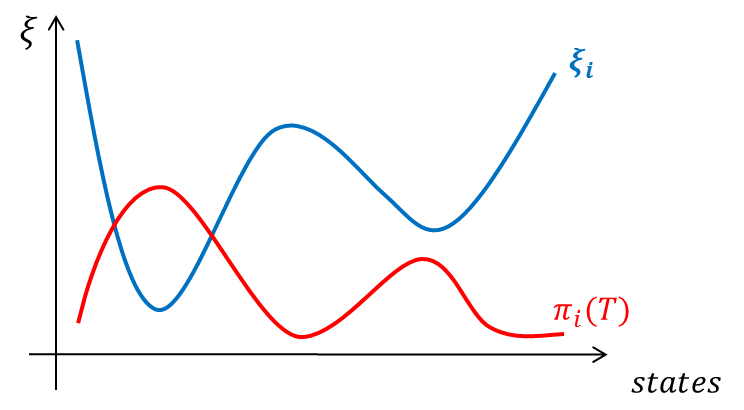
\includegraphics[scale=.7]{probabilityStatesGeneral}
\caption{Stationary distribution (red) compared with the curve of the energy of the states (blue).}
\label{figur14}
\end{figure}

Let's now analyze what happens when we start decreasing the temperature $T$. If the temperature decreases, the numerator and the denominator of $\pi_i$ decrease, but which one decreases faster? If we compute the ratio between $\pi_i$ and $\pi_j$, we get:

$$\frac{\pi_i}{\pi_j}=\frac{\frac{e^{-{\frac{\xi_i}{T}}}}{\sum_k e^{-\frac{\xi_k}{T}}}}{\frac{e^{-{\frac{\xi_j}{T}}}}{\sum_k e^{-\frac{\xi_k}{T}}}}=\frac{e^{-{\frac{\xi_i}{T}}}}{e^{-{\frac{\xi_j}{T}}}}=e^{+{\frac{\xi_j-\xi_i}{T}}}$$

If $\xi_i$ is smaller than $\xi_j$, then the difference ($\xi_j-\xi_i$) is positive. If $T$ goes to zero, this ratio goes to infinity. 

If now we say that $\xi_i$ is greater than $\xi_j$, and $T$ goes to zero, this ratio will tend to zero.

This means for $\pi_i$, that when $T$ becomes smaller, the numerator will decrease, but will decrease much faster in the states with high energy. Then, the states with higher energy will become less and less likely and the states with low energy will become more and more likely, we plotted this in Figure~\ref{figur15}.

\begin{figure}[h!]
\centering
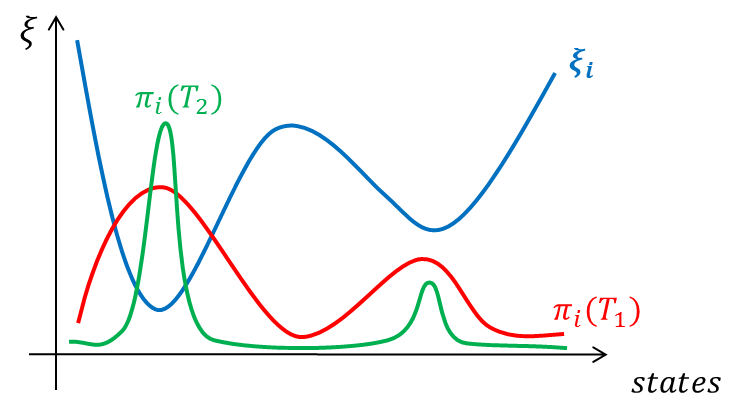
\includegraphics[scale=.7]{probabilityStates}
\caption{Stationary distribution for a temperature $T_1$ (red) compared with the Stationary distribution for a temperature $T_2 < T_1$ (green) and the curve of the energy of the states (blue).}
\label{figur15}
\end{figure}

Let's define now $H$ as the set of states with minimum energy. Then, we can prove that if you leave the temperature go to zero:

\begin{equation}
\begin{aligned}
\lim_{T \to 0} \pi_i(T) = 
\begin{cases}
\frac{1}{\mid H \mid}\ \mbox{if } i \in H\\
0\ \mbox{otherwise }
\end{cases}
\end{aligned}
\label{eq46}
\end{equation}

If the temperature reaches zero, you will be sure that your system will be in one of the global minima of the system. If you have only one global minima $\mid H \mid = 1$, the probability to be in this global minima will be equal to 1.

But we cannot decrease the temperature very fast. Because, from equation (\ref{eq40}), if $T \to 0$ the probability to move from another state with higher energy will be zero, and then we will possibly be in a local minima.

$$
\ \alpha_{ij} = 
\begin{cases}
1  & \mbox{if } \xi_{j} \leq \xi_{i}\\ 
e^{-\frac{\xi_{j}-\xi_{i}}{T}} & \mbox{if }\xi_{j} > \xi_{i}
\end{cases} 
\ \ \xrightarrow[T\to 0]{} \ \ 
\alpha_{ij} = 
\begin{cases}
1  & \mbox{if } \xi_{j} \leq \xi_{i}\\ 
0 & \mbox{if }\xi_{j} > \xi_{i}
\end{cases} 
$$

We would like to have at the beginning a temperature high enough so that we can reach the stationary distribution, and then reduce the temperature until it reaches zero.

Now we have to combine the two things:

\begin{itemize}
\item We have to run the system a long time in order to arrive to the stationary distribution.
\item And then we have to reduce the temperature.
\end{itemize}

We can think of reducing the temperature step by step. 
You start from an inicial temperature at step 0, and then you divide this temperature by $\ln(1+k)$, where $k$ is the step.

This reduction of the temperature in function of the step $k$ is defined by equation (\ref{eq47}), and is represented in Figure~\ref{figur16}.

\begin{equation}
\begin{aligned}
T(k) = \frac{T_0}{ln (1+k)}
\end{aligned}
\label{eq47}
\end{equation}

\begin{figure}[h!]
\centering
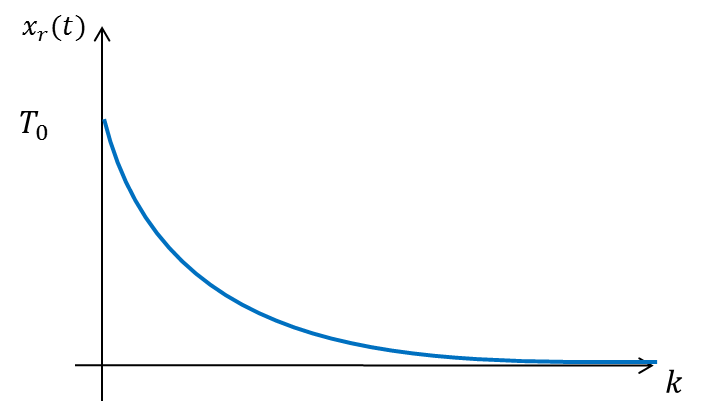
\includegraphics[scale=.7]{logDecreasingTemperature}
\caption{Decreasing of the temperature in function of the step $k$.}
\label{figur16}
\end{figure}

Then, you are guaranteed that you will assymptotically be in one of the global minima, if you execute the Algorithm 1.

\begin{algorithm}
\caption{Simmulated Annealing.}\label{euclid}
\begin{algorithmic}[1]
\Require 
\Statex $S:$ Set of states
\Statex $\textit{T}_0:$ Initial temperature
\Statex $\xi:$ Energy of the states
\Statex $\epsilon:$ tolerance
\Ensure
\Statex $i:$ State of global minima
\Procedure{SimmulAnnealing}{}
\State $i \gets \text{any state of }\textit{S}$
\State $T \gets \textit{T}_0$
\State $k \gets 1$
\While{$T > 0+\epsilon$}
	\State $j \gets \text{select a neighbor of }\textit{i}\text{ with probability }\textit{p}_{ij}$
	\If {$\xi_i > \xi_j$} 
		\State $i \gets j$
	\Else 
		\State $i \gets j\text{ with probability }\textit{e}^{-\frac{\xi_j-\xi_i}{T}}$
	\EndIf
	\State $T \gets \textit{T}_0/\ln (1+k)$
	\State $k \gets k+1$
\EndWhile
\Return $i$
\EndProcedure
\end{algorithmic}
\end{algorithm}

\begin{thebibliography}{alpha}
	
	\bibitem{Kel14} Frank Kelly and Elena Yudovina,
	\newblock Stoch	astic Networks.
	\newblock {\em Cambridge Press}, 2014.
	
\end{thebibliography}



\end{document}